% SNN-IDS: NCA (Springer) Journal Submission — Double-Blind
% Compile: pdflatex main && bibtex main && pdflatex main && pdflatex main
% TODO: Switch to Springer sn-jnl.cls and spmpsci.bst before final submission.
%       Download from: https://www.springer.com/journal/521/submission-guidelines
\documentclass[10pt,twocolumn]{article}

\usepackage[utf8]{inputenc}
\usepackage[T1]{fontenc}
\usepackage{times}
\usepackage{amsmath,amssymb}
\usepackage{graphicx}
\usepackage{booktabs}
\usepackage{hyperref}
\usepackage[margin=2cm]{geometry}
\usepackage{xcolor}
\usepackage{caption}
\usepackage{subcaption}
\usepackage{multirow}
\usepackage{array}
\usepackage{url}
\usepackage{balance}
\usepackage{tikz}
\usepackage{pgfplots}
\pgfplotsset{compat=1.18}
\usetikzlibrary{arrows.meta, positioning, calc, fit, backgrounds}

\hypersetup{colorlinks=true,linkcolor=blue,citecolor=blue,urlcolor=blue}

% Spacing
\setlength{\parskip}{0.15em}
\setlength{\abovedisplayskip}{6pt}
\setlength{\belowdisplayskip}{6pt}
\setlength{\textfloatsep}{10pt plus 2pt minus 2pt}
\setlength{\intextsep}{8pt plus 2pt minus 2pt}

% Tighter lists
\usepackage{enumitem}
\setlist[itemize]{itemsep=2pt, parsep=0pt, topsep=4pt}

\title{%
  \textbf{Practical Deployment of a Quantized SNN-Equivalent\\
  Intrusion Detector on a Commodity MCU NPU}
}

% Double-blind: author info on separate title page only.
% Real author: Hsiu-Chi Tsai, NYCU, hctsai1006@cs.nctu.edu.tw
\author{[Blinded for review]}

\date{}

\begin{document}
\maketitle

% ============================================================
\begin{abstract}
Deploying neural intrusion detection systems on microcontroller-class
hardware requires balancing classification accuracy against strict
latency, memory, and operator constraints.
This paper reports a practical deployment study of a quantized neural IDS
classifier on the STM32N6570-DK, a commodity ARM Cortex-M55 MCU with
the Neural-ART NPU (600\,GOPS INT8).
Exploiting the approximate equivalence between single-timestep
($T{=}1$) SNN inference and INT8 quantized ANN inference, we compile
a lightweight MLP to the NPU without neuromorphic hardware.
We evaluate on three standard benchmarks --- NSL-KDD (5-class),
UNSW-NB15 (10-class), and CICIDS2017 (15-class) --- with up to 20
random seeds per configuration.
INT8 NPU inference completes in 0.29--0.46\,ms
(2.7--4.2$\times$ faster than CPU-only execution), with a Flash
footprint under 140\,KB.
A 24-configuration quantization ablation on NSL-KDD shows accuracy
deviations below 1~percentage point (UNSW-NB15 is less stable),
and layer-wise analysis confirms 99\% FP32/INT8 prediction agreement
on the NSL-KDD benchmark.
We characterize the accuracy--complexity Pareto frontier across four
deployable model sizes and document that the \texttt{Floor} operator
required by QCFS activations forces CPU fallback with 17.6\% latency
overhead.
Our evaluation is bounded to classifier inference on pre-extracted
features; power consumption is estimated, not measured.
The results provide practical deployment evidence and operator-level
insight for neural IDS on commodity MCU NPUs.
\end{abstract}

\noindent\textbf{Keywords:}
intrusion detection system $\cdot$
spiking neural network $\cdot$
ANN-SNN conversion $\cdot$
quantization $\cdot$
edge AI $\cdot$
neural processing unit

% ============================================================
\section{Introduction}
\label{sec:intro}

Deep learning has transformed network intrusion detection, but deploying
these models at the network edge remains difficult. Edge IDS must operate
under tight power and latency budgets, and the dominant approach today
still relies on cloud offloading or high-end GPUs,
neither of which fits IoT or telecom CPE (customer premises equipment)
scenarios where per-device cost must stay below \$10.

Spiking neural networks offer a different compute paradigm. Because SNNs
process information as discrete spikes rather than dense floating-point
activations, they can be extremely energy-efficient when run on neuromorphic
hardware~\cite{roy2019towards}. The catch is that neuromorphic chips are not
commodity parts. Intel Loihi~\cite{davies2018loihi} is a research platform.
BrainChip Akida is available commercially but carries a price premium.
Neither is a standard MCU that an OEM can drop into a low-cost IoT gateway.

A line of theoretical work changes this picture.
Bu et al.~\cite{bu2022optimal} introduced QCFS, showing that ANN activations
can be mapped to discrete spike counts with minimal loss.
Jiang et al.~\cite{jiang2023unified} provided the first $T{=}1$ ANN--SNN
conversion framework via SlipReLU.
More recently,
Bu et al.~\cite{bu2025inference} showed that when an SNN runs for exactly
one timestep ($T{=}1$) with zero initial membrane potential, the
threshold-and-fire operation reduces to a ReLU-like clamp, making the forward
pass approximately equivalent to an INT8 quantized ANN.
The practical implication: any NPU that can execute INT8 matrix multiply
and ReLU can run an SNN-equivalent model without neuromorphic hardware.

We put this theory to the test. Using the STM32N6570-DK development board
(ARM Cortex-M55 at 800\,MHz, Neural-ART NPU rated at 600\,GOPS INT8),
we train MLP classifiers for intrusion detection on three standard
benchmarks (NSL-KDD, UNSW-NB15, and CICIDS2017), quantize them to
INT8, and deploy on the NPU through ST Edge AI Developer Cloud.
The classifier infers in 0.29--0.46\,ms (2.7--4.2$\times$ faster than
CPU-only execution) with a memory footprint under 140\,KB.
We also characterize the accuracy--complexity Pareto frontier across
four deployable model sizes (from logistic regression to the full
4-layer MLP), evaluate focal loss as a training variant for class
imbalance, and conduct a 24-configuration quantization ablation.
We focus on inference latency and memory footprint of the classifier
stage on pre-extracted flow-level features; power estimates derived from
ST's published application note are noted in Section~\ref{sec:npu} but
direct on-board measurement is deferred.
A complete end-to-end IDS pipeline (packet capture, flow aggregation,
feature extraction) is left to future work.

Our contributions:
\begin{itemize}
  \item A practical deployment study of quantized neural IDS
    classifiers on a commodity MCU NPU, covering the full pipeline from
    PyTorch training through INT8 post-training quantization to
    Neural-ART NPU execution, evaluated across three standard
    benchmarks (NSL-KDD, UNSW-NB15, CICIDS2017) with up to 20 random
    seeds per configuration.
  \item We empirically validate that $T{=}1$ SNN--ANN equivalence holds
    on commercial NPU silicon, with 99\% FP32/INT8 prediction agreement,
    layer-wise cosine analysis, and stability across 24 quantization
    configurations.
  \item We provide an operator-level deployment analysis documenting
    that QCFS-style \texttt{Floor} operations trigger CPU fallback with
    17.6\% latency overhead, and map the accuracy--complexity--latency
    Pareto frontier of NPU-deployable classifiers from logistic
    regression through a 4-layer MLP.
  \item We characterize the deployment constraints honestly: tree
    ensembles cannot run on the NPU at all, extreme minority-class
    imbalance limits recall regardless of architecture, and focal loss
    provides only marginal improvement --- establishing the practical
    boundary of neural IDS on commodity MCU NPUs.
\end{itemize}

% ============================================================
\section{Related Work}
\label{sec:related}

\subsection{SNN-Based Intrusion Detection}

Table~\ref{tab:related} summarizes prior work on neural-network-based IDS
with SNN components or edge hardware deployment.
Research on applying SNNs to network intrusion detection has grown rapidly
since 2024, though nearly all published results remain in simulation.
Wang et al.~\cite{nature2024csnn} proposed a convolutional SNN for IDS
on NSL-KDD and UNSW-NB15 in software simulation.
Prajwalasimha et al.~\cite{ieee2025event} described an event-driven
SNN-IDS and tested it in simulation.
Mustafa et al.~\cite{pmc2025hybrid} combined recurrent and spiking layers
for anomaly detection.
Karthik et al.~\cite{nature2026transformer} proposed a
transformer-spiking hybrid; all run only on GPU.

Two prior works deploy IDS on physical hardware.
Zahm et al.~\cite{zahm2024csiac} used the BrainChip Akida AKD1000
neuromorphic processor, reporting 98.4\% accuracy at approximately 1\,W.
Akida is a purpose-built neuromorphic chip (\$499 dev kit) with native
spike processing, not a general-purpose MCU.
Ngo et al.~\cite{ngo2022hhnids} deployed a lightweight MLP (1,360
parameters, 11 flow features) on the Analog Devices MAX78000, an
AI-specialized MCU with a fixed CNN accelerator.
They achieved 98.57\% on UNSW-NB15 (binary classification: normal vs.\
attack) at 18\,mW.
The MAX78000's accelerator is hard-wired for convolutional workloads;
the STM32N6 Neural-ART NPU is a programmable accelerator that supports
arbitrary operator graphs within its INT8 operator set.
Our work differs from both in targeting a general-purpose ARM Cortex-M
MCU with an attached NPU, using multi-class classification
(5-class and 10-class), and validating $T{=}1$ SNN equivalence.

\begin{table*}[t]
\centering
\caption{Comparison of neural IDS approaches with hardware deployment.
``On-chip'' indicates deployment on physical hardware. ``Task'' shows
the classification formulation. Accuracy figures are not directly
comparable across different task formulations.}
\label{tab:related}
\small
\resizebox{\textwidth}{!}{%
\begin{tabular}{@{}lllllllllll@{}}
\toprule
\textbf{Paper} & \textbf{Year} & \textbf{Dataset} & \textbf{Task} & \textbf{Model} & \textbf{Hardware} & \textbf{HW Type} & \textbf{On-chip} & \textbf{Latency} & \textbf{Energy} & \textbf{Acc.} \\
\midrule
Ngo~\cite{ngo2022hhnids} & 2022 & UNSW-NB15 & binary & MLP & MAX78000 & AI-spec.\ MCU & Yes & --- & 18\,mW$^*$ & 98.6\% \\
Wang~\cite{nature2024csnn} & 2024 & NSL-KDD & multi & Conv SNN & GPU & GPU & No & --- & --- & 94.7\% \\
Zahm~\cite{zahm2024csiac} & 2024 & UNSW-NB15 & multi & SNN & Akida AKD1000 & Neurom.\ ASIC & Yes & --- & ${\sim}$1\,W$^*$ & 98.4\% \\
Chehade~\cite{chehade2025stm32} & 2025 & VPN-nonVPN & multi & 1D-CNN & STM32F7 & MCU (no NPU) & Yes & 31\,ms & 7.86\,mJ & 96.6\% \\
Diab~\cite{diab2025rpi} & 2025 & CIC-IDS2017 & multi & LightGBM & RPi 3B+ & SBC & Yes & 27\,ms & ${\sim}$6.75\,mJ$^\ddagger$ & 95.3\% \\
Prajwal.~\cite{ieee2025event} & 2025 & NSL-KDD & multi & Event SNN & GPU & GPU & No & --- & --- & 95.4\% \\
Mustafa~\cite{pmc2025hybrid} & 2025 & UNSW-NB15 & binary & RNN-SNN & GPU & GPU & No & --- & --- & 99.7\% \\
Karthik~\cite{nature2026transformer} & 2026 & NSL-KDD & multi & Transf.-SNN & GPU & GPU & No & --- & --- & 99.2\% \\
\textbf{This work} & 2026 & NSL/UNSW/CIC & 5/10/15-cls & MLP ($T{=}1$ eq.) & STM32N6 & MCU + NPU & Yes & \textbf{0.29\,ms} & \textbf{44\,\textmu J}$^\dagger$ & 78.6/64.7/91.9\% \\
\bottomrule
\multicolumn{11}{l}{\scriptsize $^*$Power (W or mW), not per-inference energy; latency not reported.
$^\dagger$Estimated from AN5946 reference workload. $^\ddagger$Estimated from reported power and latency.}
\end{tabular}%
}
\end{table*}

\subsection{ANN-SNN Conversion}

The theory of converting a trained ANN into an equivalent SNN has matured
over several stages. Bu et al.~\cite{bu2022optimal} introduced QCFS,
a quantization-aware activation function that maps ANN activations to
discrete spike counts.
Jiang et al.~\cite{jiang2023unified} proposed a unified optimization
framework and the first $T{=}1$ conversion method (SlipReLU).
Bu et al.~\cite{bu2025inference} later analyzed the inference-scale
complexity of SNNs, establishing channel-wise threshold optimization
for $T{=}1$ conversion.
NEXUS~\cite{nexus2026} recently achieved bit-exact ANN-to-SNN equivalence
via modular arithmetic, scaling to LLaMA-2 70B.
PASCAL~\cite{pascal2025} refined multi-timestep conversion with spike
accumulation and adaptive layerwise calibration.
NeuroFlex~\cite{neuroflex2025} showed that co-executing INT8 ANN and SNN
layers on the same accelerator can cut the energy-delay product by
57--67\%.

To our knowledge, this paper provides the first empirical validation
of the $T{=}1$ equivalence on commercial NPU silicon in the IDS domain.

\subsection{Edge AI on MCU NPUs}

The STM32N6 is STMicroelectronics' first MCU with a dedicated neural
processing unit~\cite{st_neural_art}. Public deployments span computer
vision and audio processing. The NPU's hardware operator set covers
\texttt{Conv}, \texttt{Gemm}, \texttt{Relu}, \texttt{Add}, \texttt{Clip},
and \texttt{MaxPool} in INT8; operators outside this set fall back to the
Cortex-M55 CPU~\cite{st_neural_art}.
Millar et al.~\cite{millar2025munpu} benchmarked micro-NPUs including the
Neural-ART; their latency numbers provide a useful reference point.
Bruschi et al.~\cite{bruschi2024snn_mcu} deployed SNNs on ARM Cortex-M
MCUs and measured energy and latency, but targeted image classification,
not IDS, and used software SNN execution without an NPU.
To our knowledge, no prior work has deployed an IDS on a general-purpose
MCU NPU. The closest prior art (HH-NIDS~\cite{ngo2022hhnids}) used
a specialized MCU with a fixed CNN engine.
More recently, Chehade et al.~\cite{chehade2025stm32} deployed a
1D-CNN on the STM32F7 (Cortex-M7, no NPU), requiring 31\,ms and
7.86\,mJ per inference, and Diab et al.~\cite{diab2025rpi} ran
LightGBM/CNN on a Raspberry~Pi~3B+ (27\,ms).

% ============================================================
\section{Background}
\label{sec:background}

\subsection{\texorpdfstring{$T{=}1$}{T=1} SNN--ANN Equivalence}

A Leaky Integrate-and-Fire (LIF) neuron with membrane potential $V$,
weight matrix $\mathbf{W}$, and threshold $\theta$ operates as:
%
\begin{align}
  V[t] &= \beta \cdot V[t{-}1] + \mathbf{W} \cdot \mathbf{x}[t] \label{eq:lif1}\\
  S[t] &= \Theta(V[t] - \theta) \label{eq:lif2}
\end{align}
%
where $\Theta$ is the Heaviside step function and $\beta$ is the leak factor.
At $T{=}1$ with zero initial state ($V[0]=0$), the leak term
$\beta \cdot V[0]$ vanishes regardless of $\beta$, so
Eq.~\ref{eq:lif1} simplifies to $V[1] = \mathbf{W} \cdot \mathbf{x}$.

Multiple works have established that INT8 post-training quantization
produces a discretization that closely approximates the threshold-and-fire
operation~\cite{bu2022optimal, jiang2023unified, bu2025inference}.
In practice, any NPU executing INT8 \texttt{Gemm} + \texttt{Relu}
is performing SNN-equivalent computation, with accuracy gaps typically
below 1\,pp on standard benchmarks.

\subsection{QCFS Activation}

QCFS~\cite{bu2022optimal} maps ANN activations to discrete spike counts:
$\text{QCFS}(x) = \lfloor \text{clip}(x/s,\, 0,\, L) \rfloor \cdot s$,
where $s{=}\theta/L$ is the quantization step and $L$ is the number of
levels. Its ONNX graph requires \texttt{Floor}, which is absent from
the Neural-ART operator set (Section~\ref{sec:npu}).

\subsection{STM32N6 Neural-ART NPU}

The STM32N6570-DK pairs an ARM Cortex-M55 at 800\,MHz with ST's Neural-ART
NPU, rated at 600\,GOPS for INT8 workloads and 3\,TOPS/W
efficiency~\cite{st_neural_art}.
The board includes 4.2\,MB internal SRAM and 128\,MB external NOR Flash.
Table~\ref{tab:opmap} lists the operator-level mapping.
The NPU natively supports \texttt{Conv}, \texttt{Gemm}, \texttt{Relu},
\texttt{Add}, \texttt{Clip}, and \texttt{MaxPool} in INT8.
Operators outside this set are dispatched to the Cortex-M55 CPU,
incurring cache-maintenance overhead for each
NPU$\leftrightarrow$CPU data transfer.
All hidden dimensions are powers of two (256, 128), avoiding a known
Neural-ART compiler issue with prime-number channel
counts~\cite{st_neural_art}.

\begin{table}[t]
\centering
\caption{Operator mapping to NPU execution epochs. ReLU INT8 achieves
near-100\% NPU utilization; QCFS INT8 forces CPU fallback at every
\texttt{Floor} invocation.}
\label{tab:opmap}
\small
\resizebox{\columnwidth}{!}{%
\begin{tabular}{@{}llcl@{}}
\toprule
\textbf{ONNX Operator} & \textbf{NPU?} & \textbf{Epoch} & \textbf{Notes} \\
\midrule
\texttt{Gemm} (INT8)  & Yes & HW & Fused weight + bias \\
\texttt{Relu}          & Yes & HW & Fused with Gemm \\
\texttt{Clip}          & Yes & HW & Used by QCFS \\
\texttt{Floor}         & No  & SW & CPU fallback (+0.08\,ms) \\
\texttt{QuantizeLinear}   & Yes & HW/Hyb & Model boundary \\
\texttt{DequantizeLinear} & Yes & HW/Hyb & Model boundary \\
\bottomrule
\end{tabular}%
}
\end{table}

% ============================================================
\section{Method}
\label{sec:method}

Figure~\ref{fig:pipeline} shows the deployment pipeline.
Both paths share the same training and export procedure; they diverge
only in the activation function.

\begin{figure*}[t]
\centering
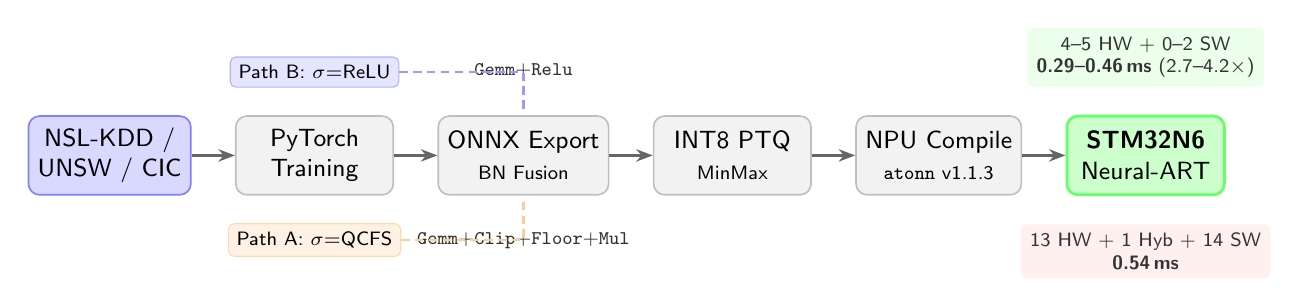
\begin{tikzpicture}[
  node distance=0.5cm and 0.55cm,
  box/.style={draw, rounded corners=4pt, minimum height=1.0cm,
              minimum width=2.0cm, align=center, font=\small\sffamily,
              line width=0.6pt},
  data/.style={box, fill=blue!15, draw=blue!50},
  proc/.style={box, fill=gray!10, draw=gray!50},
  hw/.style={box, fill=green!20, draw=green!60, line width=1pt},
  arr/.style={-{Stealth[length=6pt]}, thick, draw=black!60},
  pathlbl/.style={font=\scriptsize\sffamily, rounded corners=2pt,
                  inner sep=3pt},
  reslbl/.style={font=\scriptsize\sffamily, align=center, text=black!80},
]
% Main pipeline
\node[data] (dataset) {NSL-KDD /\\UNSW / CIC};
\node[proc, right=of dataset] (train) {PyTorch\\Training};
\node[proc, right=of train] (export) {ONNX Export\\{\scriptsize BN Fusion}};
\node[proc, right=of export] (ptq) {INT8 PTQ\\{\scriptsize MinMax}};
\node[proc, right=of ptq] (compile) {NPU Compile\\{\scriptsize\texttt{atonn} v1.1.3}};
\node[hw, right=of compile] (npu) {\textbf{STM32N6}\\Neural-ART};

\draw[arr] (dataset) -- (train);
\draw[arr] (train) -- (export);
\draw[arr] (export) -- (ptq);
\draw[arr] (ptq) -- (compile);
\draw[arr] (compile) -- (npu);

% Path B label (top)
\node[pathlbl, fill=blue!10, draw=blue!30,
      above=0.35cm of train] (pathb) {Path B: $\sigma{=}\text{ReLU}$};
% Path A label (bottom)
\node[pathlbl, fill=orange!10, draw=orange!30,
      below=0.35cm of train] (patha) {Path A: $\sigma{=}\text{QCFS}$};

% ONNX operators
\node[reslbl, above=0.35cm of export]
  {\texttt{Gemm}+\texttt{Relu}};
\node[reslbl, below=0.35cm of export]
  {\texttt{Gemm}+\texttt{Clip}+\texttt{Floor}+\texttt{Mul}};

% NPU epoch result
\node[reslbl, fill=green!8, rounded corners=2pt,
      above=0.35cm of npu]
  {4--5 HW + 0--2 SW\\\textbf{0.29--0.46\,ms} (2.7--4.2$\times$)};
\node[reslbl, fill=red!6, rounded corners=2pt,
      below=0.35cm of npu]
  {13 HW + 1 Hyb + 14 SW\\\textbf{0.54\,ms}};

\draw[densely dashed, blue!40, thick]
  (pathb.east) -| ($(export.north)+(0,0.05)$);
\draw[densely dashed, orange!40, thick]
  (patha.east) -| ($(export.south)-(0,0.05)$);
\end{tikzpicture}
\caption{Deployment pipeline. Path~B (ReLU) produces a Gemm+Relu
graph that maps to the NPU. Path~A (QCFS) adds Floor, which falls
back to CPU.}
\label{fig:pipeline}
\end{figure*}

\subsection{Model Architecture}

We use a four-layer MLP with BatchNorm:
%
\begin{align*}
  &\texttt{Lin}(d {\to} 256) \to \texttt{BN} \to \sigma \to
   \texttt{Lin}(256 {\to} 256) \to \texttt{BN} \to \sigma \\
  &\to \texttt{Lin}(256 {\to} 128) \to \texttt{BN} \to \sigma \to
   \texttt{Lin}(128 {\to} C)
\end{align*}
%
where $d$ is the input dimension (41 for NSL-KDD, 34 for UNSW-NB15,
69 for CICIDS2017),
$C$ is the number of classes (5, 10, or 15),
and $\sigma$ is ReLU (Path~B) or QCFS $L{=}4$ (Path~A).
The full model has ${\sim}$110K parameters.
At ONNX export, BatchNorm is folded into the preceding Linear layer.
To map the accuracy--complexity Pareto frontier, we also evaluate
three smaller deployable architectures: logistic regression
($\texttt{Lin}(d{\to}C)$), a 2-layer MLP ($64{\to}64{\to}C$),
and a 2-layer MLP ($128{\to}64{\to}C$).
All use the same training protocol and are eligible for NPU
acceleration.

\subsection{Datasets}

\textbf{NSL-KDD}~\cite{tavallaee2009nslkdd} contains 125,973 training and
22,544 test instances with 41 features. We use 5-class grouping:
\textit{normal}, \textit{DoS}, \textit{Probe}, \textit{R2L}, \textit{U2R}.
Three categorical features are label-encoded; 38 continuous features
are z-score normalized using training-set statistics.

\textbf{UNSW-NB15}~\cite{moustafa2015unsw} contains 175,341 training and
82,332 test instances with 34 features and 10 attack categories:
\textit{Analysis}, \textit{Backdoor}, \textit{DoS}, \textit{Exploits},
\textit{Fuzzers}, \textit{Generic}, \textit{Normal},
\textit{Reconnaissance}, \textit{Shellcode}, \textit{Worms}.
Three categorical features (\texttt{proto}, \texttt{service},
\texttt{state}) are label-encoded; remaining features are z-score
normalized.

\textbf{CICIDS2017}~\cite{sharafaldin2018cicids} contains 2,830,743
flow records with 78 CICFlowMeter features and 15 classes (BENIGN
80.3\%, plus 14 attack types). We use 80/20 stratified random split
(no standard split exists for this dataset).
Identifier columns (Flow ID, Source/Destination IP and Port) are
dropped. NaN and Inf values are replaced with zero.
Constant-valued columns and negative byte/packet counts (a known
CICFlowMeter bug) are clipped to zero.
Two classes are extremely rare: Heartbleed (11~samples) and
Infiltration (36~samples).

\subsection{Training}

Both paths use Adam ($\text{lr}=10^{-3}$, weight decay $10^{-5}$),
cosine annealing over 80 epochs, batch size 512, and inverse-frequency
class weighting.
As a training variant, we also evaluate focal
loss~\cite{lin2017focal}: $\text{FL}(p_t) = -\alpha_t (1-p_t)^\gamma
\log(p_t)$ with $\gamma \in \{1, 2, 3\}$ ($\gamma{=}0$ reduces to
weighted cross-entropy) and $\alpha$ set to inverse-frequency weights.
All experiments are repeated with multiple random seeds
(NSL-KDD and UNSW-NB15: 20 seeds; CICIDS2017: 10 seeds);
we report mean $\pm$ standard deviation.
Training uses PyTorch 2.10 on a GPU workstation.

\subsection{INT8 Post-Training Quantization}

FP32 ONNX models are quantized to INT8 using ONNX Runtime static
quantization. The default configuration uses MinMax calibration on 1,000
randomly sampled training instances with per-tensor quantization.
Section~\ref{sec:quant_ablation} explores the sensitivity to calibration
method, granularity, and sample size.

\subsection{NPU Compilation}

Models are compiled for the STM32N6570-DK using ST Edge AI Developer Cloud
v4.0.0 (compiler: Neural-ART \texttt{atonn} v1.1.3). The compiler
partitions the ONNX graph into NPU-executable epochs (hardware or hybrid)
and CPU-only epochs (software).

% ============================================================
\section{Experiments}
\label{sec:experiments}

\subsection{Multi-Seed Classification Results}

\begin{table}[t]
\centering
\caption{Test accuracy (\%, mean$\pm$std) on NSL-KDD ($n{=}20$ seeds),
UNSW-NB15 ($n{=}20$), and CICIDS2017 ($n{=}10$). Best per dataset in \textbf{bold}. NPU = deployable on
Neural-ART NPU.}
\label{tab:accuracy}
\small
\resizebox{\columnwidth}{!}{%
\begin{tabular}{@{}llcccc@{}}
\toprule
\textbf{Dataset} & \textbf{Model} & \textbf{NPU} & \textbf{Overall} & \textbf{Macro F1} & \textbf{MCC} \\
\midrule
\multirow{4}{*}{NSL-KDD}
  & ReLU MLP     & Yes & \textbf{78.57$\pm$1.28} & \textbf{58.91$\pm$2.80} & \textbf{0.688$\pm$0.018} \\
  & QCFS $L{=}4$ & Partial & 78.14$\pm$1.08 & 58.28$\pm$2.70 & --- \\
  & Rand.\ Forest & No & 73.84$\pm$0.19 & 47.13$\pm$0.33 & --- \\
  & XGBoost      & No & 76.86$\pm$0.00 & 55.52$\pm$0.00 & --- \\
\midrule
\multirow{3}{*}{UNSW-NB15}
  & ReLU MLP     & Yes & 64.67$\pm$0.55 & 40.18$\pm$1.02 & 0.582$\pm$0.005 \\
  & Rand.\ Forest & No & \textbf{69.46$\pm$0.10} & \textbf{48.63$\pm$0.38} & --- \\
  & XGBoost      & No & 67.10$\pm$0.00 & 47.46$\pm$0.00 & --- \\
\midrule
CICIDS2017
  & ReLU MLP     & Yes & 91.89$\pm$1.21 & 56.35$\pm$2.80 & 0.813$\pm$0.021 \\
\bottomrule
\end{tabular}%
}
\end{table}

Table~\ref{tab:accuracy} reports classification results.
On NSL-KDD (20 seeds), the ReLU MLP achieves the best overall accuracy
($78.57{\pm}1.28$\%) and macro F1 ($58.91{\pm}2.80$\%), outperforming
both tree baselines and QCFS.
A Wilcoxon signed-rank test yields $p{=}0.227$ for overall accuracy
and $p{=}0.729$ for macro F1 (neither significant at $\alpha{=}0.05$),
confirming that ReLU and QCFS are statistically equivalent on this
benchmark --- consistent with the $T{=}1$ equivalence hypothesis.

On UNSW-NB15 (10-class, 20 seeds), the MLP achieves $64.67{\pm}0.55$\% overall
accuracy, lower than Random Forest ($69.46{\pm}0.10$\%). However, the
MLP achieves the highest macro accuracy ($61.18{\pm}0.62$\%), which
reflects better balance across minority classes from inverse-frequency
weighting.
The gap in overall accuracy reflects the difficulty of UNSW-NB15's
10-class problem with extreme imbalance (Worms: 130 training / 44 test
samples vs.\ Normal: 56,000 training).

Table~\ref{tab:security_metrics} presents additional security-relevant
metrics for the ReLU MLP across all three datasets.
ROC-AUC (macro OVR) ranges from 0.858 on NSL-KDD to 0.992 on
CICIDS2017, confirming strong ranking ability despite the moderate
macro F1 scores.
MCC ranges from 0.582 (UNSW, 10-class) to 0.813 (CICIDS, 15-class),
reflecting the interaction between dataset size and class separability.

\begin{table}[t]
\centering
\caption{Security-relevant metrics for ReLU MLP (mean$\pm$std).
NSL-KDD and UNSW-NB15: $n{=}20$ seeds; CICIDS2017: $n{=}10$.
BA = balanced accuracy, WF1 = weighted F1.}
\label{tab:security_metrics}
\small
\resizebox{\columnwidth}{!}{%
\begin{tabular}{@{}lcccc@{}}
\toprule
\textbf{Dataset} & \textbf{BA (\%)} & \textbf{MCC} & \textbf{ROC-AUC} & \textbf{WF1 (\%)} \\
\midrule
NSL-KDD   & 57.92$\pm$1.98 & 0.688$\pm$0.018 & 0.864$\pm$0.018 & 76.97$\pm$1.71 \\
UNSW-NB15 & 61.18$\pm$0.62 & 0.582$\pm$0.005 & 0.943$\pm$0.002 & 70.48$\pm$0.51 \\
CICIDS2017& 87.58$\pm$0.80 & 0.813$\pm$0.021 & 0.992$\pm$0.004 & 94.03$\pm$0.92 \\
\bottomrule
\end{tabular}%
}
\end{table}

\subsection{Per-Class Performance}

\begin{table}[t]
\centering
\caption{Per-class metrics (\%, mean$\pm$std, $n{=}20$) for ReLU MLP on NSL-KDD.
P = precision, R = recall, F1 = F1-score.}
\label{tab:perclass_nslkdd}
\small
\begin{tabular}{@{}lcccc@{}}
\toprule
\textbf{Class} & \textbf{P} & \textbf{R} & \textbf{F1} & \textbf{Support} \\
\midrule
DoS     & 95.7$\pm$0.9 & 79.7$\pm$2.3 & 86.9$\pm$1.3 & 7,458 \\
Probe   & 77.7$\pm$1.9 & 69.2$\pm$4.9 & 73.1$\pm$2.9 & 2,421 \\
R2L     & 93.0$\pm$2.3 & 25.3$\pm$9.4 & 39.0$\pm$11.4 & 2,754 \\
U2R     & 11.8$\pm$8.0 & 19.0$\pm$3.8 & 13.2$\pm$3.4 & 200 \\
Normal  & 71.9$\pm$1.4 & 96.4$\pm$0.5 & 82.4$\pm$0.9 & 9,711 \\
\bottomrule
\end{tabular}
\end{table}

Table~\ref{tab:perclass_nslkdd} shows per-class metrics on NSL-KDD.
DoS and Normal achieve strong F1 ($>82$\%), but R2L and U2R remain
challenging. R2L exhibits high precision (93.0\%) but low recall
(25.3\%), indicating that the model correctly identifies R2L when it
predicts the class but misses most R2L samples.
U2R has only 52 training samples (0.04\% of the training set);
no amount of class weighting can fully compensate.
Figure~\ref{fig:cm_nslkdd} visualizes the confusion pattern:
R2L samples overwhelmingly fall into the Normal bin (63.2\%),
and U2R scatters across Probe (45.4\%) and Normal (29.2\%).

\begin{figure}[t]
\centering
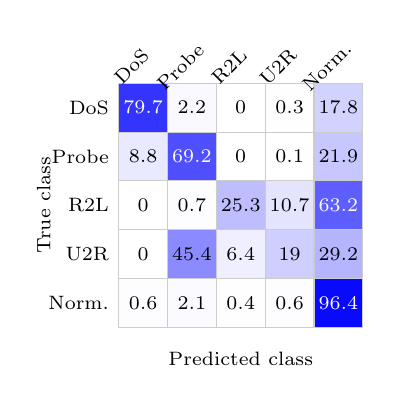
\begin{tikzpicture}[scale=0.62, every node/.style={font=\scriptsize}]
  % Color helper: value 0-100 maps to white(0)..blue(100)
  \foreach \row/\rname [count=\ri from 0] in {
    {79.7, 2.2, 0.0, 0.3,17.8}/DoS,
    { 8.8,69.2, 0.0, 0.1,21.9}/Probe,
    { 0.0, 0.7,25.3,10.7,63.2}/R2L,
    { 0.0,45.4, 6.4,19.0,29.2}/U2R,
    { 0.6, 2.1, 0.4, 0.6,96.4}/Norm.} {
    \foreach \val [count=\ci from 0] in \row {
      \pgfmathsetmacro{\intensity}{\val}
      \pgfmathsetmacro{\textcol}{ifthenelse(\intensity>55,"white","black")}
      \fill[blue!\intensity!white] (\ci,-\ri) rectangle ++(1,-1);
      \draw[gray!40] (\ci,-\ri) rectangle ++(1,-1);
      \node[text=\textcol] at (\ci+0.5,-\ri-0.5) {\pgfmathprintnumber[fixed,precision=1]{\val}};
    }
    % Row label (true class)
    \node[anchor=east] at (0,-\ri-0.5) {\rname};
  }
  % Column labels (predicted)
  \foreach \cname [count=\ci from 0] in {DoS,Probe,R2L,U2R,Norm.} {
    \node[anchor=south, rotate=45] at (\ci+0.5,0.1) {\cname};
  }
  % Axis labels
  \node[rotate=90, anchor=south] at (-1.2,-2.5) {True class};
  \node[anchor=north] at (2.5,-5.3) {Predicted class};
\end{tikzpicture}
\caption{Normalized confusion matrix (\%, 20-seed mean) for ReLU MLP
on NSL-KDD. R2L$\to$Normal (63.2\%) and U2R$\to$Probe (45.4\%) are
the dominant misclassification patterns.}
\label{fig:cm_nslkdd}
\end{figure}

Table~\ref{tab:perclass_unsw} shows per-class results on UNSW-NB15.
Generic dominates (F1$=$97.9\%), while extreme minority classes
collapse: Worms (44 test samples, F1$=$9.1\%), Analysis (F1$=$2.9\%).
Normal achieves 98.7\% precision but only 57.7\% recall ---
inverse-frequency weighting shifts predictions toward attack
categories at the expense of the majority class.

\begin{table}[t]
\centering
\caption{Per-class metrics (\%, mean$\pm$std, $n{=}20$) for ReLU MLP on UNSW-NB15.
Classes sorted by F1 descending.}
\label{tab:perclass_unsw}
\small
\resizebox{\columnwidth}{!}{%
\begin{tabular}{@{}lcccc@{}}
\toprule
\textbf{Class} & \textbf{P} & \textbf{R} & \textbf{F1} & \textbf{Support} \\
\midrule
Generic        & 99.8$\pm$0.1 & 96.1$\pm$0.3 & 97.9$\pm$0.2 & 18,871 \\
Reconnaissance & 68.3$\pm$5.3 & 83.4$\pm$1.0 & 75.0$\pm$3.1 & 3,496 \\
Normal         & 98.7$\pm$0.3 & 57.7$\pm$0.6 & 72.8$\pm$0.4 & 37,000 \\
Exploits       & 78.9$\pm$1.2 & 49.5$\pm$1.3 & 60.8$\pm$0.7 & 11,132 \\
Fuzzers        & 27.2$\pm$0.5 & 64.8$\pm$2.2 & 38.3$\pm$0.6 & 6,062 \\
DoS            & 29.5$\pm$3.3 & 14.6$\pm$7.2 & 18.5$\pm$5.6 & 4,089 \\
Shellcode      &  8.7$\pm$1.1 & 86.4$\pm$3.6 & 15.8$\pm$1.8 & 378 \\
Backdoor       &  5.7$\pm$0.5 & 65.5$\pm$17.6 & 10.5$\pm$0.9 & 583 \\
Worms          &  4.9$\pm$1.7 & 81.8$\pm$5.4 &  9.1$\pm$3.0 & 44 \\
Analysis       &  1.7$\pm$1.7 & 12.0$\pm$17.2 &  2.9$\pm$3.0 & 677 \\
\bottomrule
\end{tabular}%
}
\end{table}

\subsection{CICIDS2017 Results}

On CICIDS2017 (15-class, 2.83M records), the ReLU MLP achieves
$91.89{\pm}1.21$\% overall accuracy, $87.58{\pm}0.80$\% macro
accuracy, and MCC of $0.813{\pm}0.021$ (Table~\ref{tab:accuracy}).
The ROC-AUC (macro) reaches 0.992, indicating strong ranking ability.
The gap between weighted F1 (94.0\%) and macro F1 (56.4\%) reflects
the familiar imbalance pattern: dominant classes (DDoS F1$=$98.1\%,
BENIGN 94.7\%, DoS~Hulk 91.2\%) drive high weighted performance
while rare classes collapse (Web Attack SQL Injection: 4~test
samples, F1$=$1.4\%; Bot: F1$=$6.3\%).
This 15-class formulation is substantially harder than binary or
5-class: Diab et al.~\cite{diab2025rpi} report 95.3\% on the
same dataset with multi-class LightGBM on a Raspberry~Pi, but
with fewer class distinctions.
The Pareto, focal loss, quantization ablation, and NPU benchmark
analyses (Sections~\ref{sec:pareto}--\ref{sec:npu}) are reported
on NSL-KDD and UNSW-NB15 only; CICIDS2017 hardware deployment
is left to future work pending ST Cloud benchmarking.

\subsection{Accuracy--Complexity Pareto Frontier}
\label{sec:pareto}

\begin{table}[t]
\centering
\caption{Accuracy--complexity Pareto frontier (\%, mean$\pm$std).
Baselines: 10 seeds; full MLP: 20 seeds (NSL-KDD) / 20 seeds (UNSW).
All models are NPU-deployable (Gemm+Relu only).}
\label{tab:pareto}
\small
\resizebox{\columnwidth}{!}{%
\begin{tabular}{@{}llcccc@{}}
\toprule
\textbf{Dataset} & \textbf{Model} & \textbf{Params} & \textbf{OA (\%)} & \textbf{MF1 (\%)} & \textbf{MCC} \\
\midrule
\multirow{4}{*}{NSL-KDD}
  & LogReg           &    210 & 78.42$\pm$0.56 & 60.40$\pm$1.24 & 0.686$\pm$0.009 \\
  & MLP 64-64        &  7,429 & 78.77$\pm$1.42 & 58.66$\pm$3.09 & 0.690$\pm$0.020 \\
  & MLP 128-64       & 14,341 & 78.40$\pm$1.59 & 57.49$\pm$1.97 & 0.685$\pm$0.023 \\
  & MLP 256-256-128  &111,365 & \textbf{78.57$\pm$1.28} & \textbf{58.91$\pm$2.80} & \textbf{0.688$\pm$0.018} \\
\midrule
\multirow{4}{*}{UNSW}
  & LogReg           &    350 & 51.81$\pm$0.27 & 29.25$\pm$0.46 & 0.439$\pm$0.003 \\
  & MLP 64-64        &  7,306 & 64.52$\pm$0.39 & 39.94$\pm$0.76 & 0.581$\pm$0.004 \\
  & MLP 128-64       & 13,770 & 64.72$\pm$0.41 & 40.05$\pm$0.65 & 0.583$\pm$0.004 \\
  & MLP 256-256-128  &110,218 & \textbf{64.67$\pm$0.55} & \textbf{40.18$\pm$1.02} & \textbf{0.582$\pm$0.005} \\
\bottomrule
\end{tabular}%
}
\end{table}

Table~\ref{tab:pareto} maps the accuracy--complexity Pareto frontier.
On NSL-KDD, logistic regression (210~parameters) achieves 78.42\%
overall accuracy, only 0.44\,pp below the full MLP (111K~parameters).
This is a 530$\times$ parameter reduction with negligible accuracy
loss, because the 41-dimensional 5-class problem is nearly linearly
separable.
On UNSW-NB15, the gap is large: logistic regression falls to 51.81\%
(vs.\ 64.67\% for the full MLP), confirming that the 10-class problem
benefits from nonlinear hidden layers.
Between the two-layer MLPs (7K--14K parameters), accuracy plateaus
with diminishing returns beyond 64\%.
All four architectures use only \texttt{Gemm} and \texttt{Relu}
operators and are thus eligible for full NPU acceleration.
Their INT8 ONNX sizes range from 1.7\,KB (LogReg) to 18\,KB
(MLP~128-64).

\subsection{Focal Loss Ablation}
\label{sec:focal}

\begin{table}[t]
\centering
\caption{Focal loss ablation (\%, mean$\pm$std, $n{=}10$ seeds). $\gamma{=}0$
is weighted cross-entropy (baseline). Best per dataset in \textbf{bold}.}
\label{tab:focal}
\small
\begin{tabular}{@{}llcc@{}}
\toprule
\textbf{Dataset} & $\gamma$ & \textbf{OA (\%)} & \textbf{Macro F1 (\%)} \\
\midrule
\multirow{4}{*}{NSL-KDD}
  & 0 (CE) & 78.86$\pm$1.32 & 59.20$\pm$2.80 \\
  & 1      & \textbf{79.37$\pm$1.73} & \textbf{61.70$\pm$3.36} \\
  & 2      & 79.38$\pm$1.07 & 60.52$\pm$2.60 \\
  & 3      & 78.07$\pm$1.32 & 58.99$\pm$3.04 \\
\midrule
\multirow{4}{*}{UNSW}
  & 0 (CE) & \textbf{64.75$\pm$0.61} & \textbf{40.29$\pm$0.90} \\
  & 1      & 64.40$\pm$0.39 & 39.86$\pm$0.86 \\
  & 2      & 64.26$\pm$0.62 & 39.57$\pm$0.85 \\
  & 3      & 64.33$\pm$0.43 & 39.87$\pm$0.91 \\
\bottomrule
\end{tabular}
\end{table}

Table~\ref{tab:focal} presents the focal loss ablation.
On NSL-KDD, $\gamma{=}1$ yields the best macro F1 (61.70\% vs.\
59.20\% baseline); minority-class recall also improves
(R2L: 33.4\% vs.\ 25.0\%, U2R: 20.6\% vs.\ 18.6\%).
However, none of these differences reach statistical significance
(Wilcoxon signed-rank $p{=}0.16$ for MF1).
On UNSW-NB15, focal loss provides no improvement: the baseline
weighted cross-entropy ($\gamma{=}0$) achieves the highest OA
and MF1, and $\gamma{=}2$ significantly degrades OA
($p{=}0.037$).
Focal loss cannot overcome data scarcity:
when minority classes have very few training samples
(NSL-KDD U2R: 52 training; UNSW Worms: 130 training; CICIDS Heartbleed: ${\sim}$9 training),
no loss function compensates for the lack of examples.

\subsection{Layer-Wise FP32 vs INT8 Equivalence}
\label{sec:layerwise}

\begin{table}[t]
\centering
\caption{Layer-wise comparison between FP32 and INT8 ONNX models
on 1,000 NSL-KDD test samples. Cosine similarity is computed on
flattened activation vectors.}
\label{tab:layerwise}
\small
\begin{tabular}{@{}lcccc@{}}
\toprule
\textbf{Layer} & \textbf{Shape} & \textbf{Cosine Sim} & \textbf{MAE} & \textbf{$L_\infty$} \\
\midrule
Relu\_0 (256) & $1000{\times}256$ & 0.667 & 0.435 & 43.7 \\
Relu\_1 (256) & $1000{\times}256$ & 0.655 & 0.438 & 62.6 \\
Relu\_2 (128) & $1000{\times}128$ & 0.683 & 0.400 & 65.2 \\
Logits (5)    & $1000{\times}5$   & \textbf{0.978} & 0.103 & 19.8 \\
\bottomrule
\end{tabular}
\end{table}

Table~\ref{tab:layerwise} presents layer-wise activation comparison
between the FP32 and INT8 models.
Individual hidden layers show moderate cosine similarity (0.65--0.68)
due to per-neuron quantization noise, but the logit layer recovers to
0.978.
The overall prediction agreement is \textbf{99.0\%}
(per-class: Normal 99.8\%, DoS 99.4\%, R2L 99.3\%, Probe 95.4\%,
U2R 85.7\%).
INT8 quantization introduces bounded perturbation
at each layer, but the accumulated effect on the final classification decision
is negligible.
From the $T{=}1$ SNN perspective, this means the quantized SNN
(INT8 model) closely reproduces the firing decisions of the original SNN
(FP32 ReLU model with $V[0]{=}0$).

\subsection{Quantization Ablation}
\label{sec:quant_ablation}

\begin{table}[t]
\centering
\caption{INT8 quantization ablation on NSL-KDD (8 representative rows
of 24 total). FP32 baseline: 76.45\% (seed 42, used for ONNX export).
$\Delta$ = FP32 $-$ INT8 (positive = degradation).
All 24 configurations show $|\Delta| < 1$\,pp.}
\label{tab:quant_ablation}
\small
\begin{tabular}{@{}lcccc@{}}
\toprule
\textbf{Method} & \textbf{Granularity} & \textbf{Cal.\ Samples} & \textbf{INT8 \%} & \textbf{$\Delta$} \\
\midrule
MinMax     & per-tensor  & 100   & 76.59 & $-$0.14 \\
MinMax     & per-tensor  & 1000  & 76.38 & +0.08 \\
MinMax     & per-tensor  & 5000  & 77.27 & $-$0.82 \\
MinMax     & per-channel & 1000  & 76.51 & $-$0.05 \\
\midrule
Entropy    & per-tensor  & 1000  & 76.38 & +0.08 \\
Entropy    & per-channel & 1000  & 76.51 & $-$0.05 \\
\midrule
Percentile & per-tensor  & 1000  & 76.39 & +0.07 \\
Percentile & per-channel & 1000  & 76.28 & +0.17 \\
\bottomrule
\end{tabular}
\end{table}

Table~\ref{tab:quant_ablation} shows a representative subset of the full
24-configuration ablation (3 methods $\times$ 2 granularities $\times$
4 sample sizes; full results in the supplementary material).
On NSL-KDD, all configurations deviate from FP32 by at most
0.82\,pp, and several INT8 configurations actually \emph{improve} over
FP32 (likely due to regularization effects of quantization noise).
This stability is expected for a small model (111K parameters, 4 layers):
the quantization grid resolution (256 INT8 levels) is sufficient to
represent the narrow activation distributions of a shallow MLP.

\emph{Caveat}: The same ablation on UNSW-NB15 reveals fragility ---
accuracy drops range from 0.85\,pp (100 calibration samples) to
11.82\,pp (Percentile, per-channel, 500 samples).
The UNSW model operates near the decision boundary (FP32 65.42\%
on a 10-class problem), and larger calibration sets paradoxically
increase quantization error, likely because the calibration range
estimates over-fit to activation outliers from minority classes.
For deployment, the NSL-KDD-validated MinMax per-tensor configuration
(100--1000 samples) is the recommended default.

\subsection{NPU Hardware Benchmark}
\label{sec:npu}

\begin{table}[t]
\centering
\caption{Hardware benchmark on STM32N6570-DK (Cortex-M55 @ 800\,MHz +
Neural-ART NPU). HW = NPU-only epochs, Hyb = mixed, SW = CPU-only.}
\label{tab:npu}
\small
\resizebox{\columnwidth}{!}{%
\begin{tabular}{@{}llccccccc@{}}
\toprule
\textbf{Model} & \textbf{Dataset} & \textbf{Time} & \textbf{HW} & \textbf{Hyb} & \textbf{SW} & \textbf{Flash} & \textbf{RAM} \\
 & & \textbf{(ms)} & & & & \textbf{(KB)} & \textbf{(KB)} \\
\midrule
ReLU FP32 & NSL-KDD & 1.24 & 0 & 0 & 11 & 466.4 & 2.17 \\
ReLU INT8 & NSL-KDD & 0.46 & 5 & 1 & 2 & 137.7 & 1.25 \\
\midrule
ReLU FP32 & UNSW-NB15 & 1.23 & 0 & 0 & 11 & 461.9 & 2.14 \\
ReLU INT8 & UNSW-NB15 & \textbf{0.29} & 4 & 0 & 0 & 120.6 & 0.50 \\
\midrule
QCFS INT8 & NSL-KDD & 0.54 & 13 & 1 & 14 & 138.0 & 2.00 \\
\bottomrule
\end{tabular}%
}
\end{table}

Table~\ref{tab:npu} presents measurements from the STM32N6570-DK.
We first establish a CPU baseline: the same ReLU MLP compiled as FP32
runs entirely on the Cortex-M55 CPU (0~HW epochs, 11~SW epochs) at
1.24\,ms (NSL-KDD) and 1.23\,ms (UNSW-NB15).

INT8 quantization combined with NPU acceleration yields
\textbf{2.7$\times$} speedup on NSL-KDD (1.24$\to$0.46\,ms) and
\textbf{4.2$\times$} on UNSW-NB15 (1.23$\to$0.29\,ms).
The larger speedup on UNSW-NB15 reflects 100\% NPU execution
(4~HW epochs, zero SW fallback), while NSL-KDD retains 2~SW epochs.
Flash memory shrinks 3.4--3.8$\times$ from FP32 to INT8.
ST Application Note AN5946 reports ${\sim}150$\,mW average power during
NPU inference at nominal frequency~\cite{st_an5946}.
Combining this with our measured latency yields an estimated
${\sim}69$\,\textmu J/inference (NSL-KDD) and
${\sim}44$\,\textmu J/inference (UNSW-NB15).
These figures are derived from the reference workload in AN5946, not
direct measurement of our model, and should be validated with
on-board instrumentation.

QCFS INT8 runs \texttt{Gemm} on the NPU but each \texttt{Floor}
triggers a CPU fallback via \mbox{\texttt{DequantizeLinear}}
$\to$ \mbox{\texttt{Floor(float)}} $\to$ \mbox{\texttt{QuantizeLinear}},
adding 0.08\,ms (+17.6\%) over ReLU INT8.
The \texttt{Floor} operator is absent from ST's published
NPU operator list~\cite{st_neural_art}.

\subsection{Tree-Based Baseline Comparison}

Random Forest (100 trees, max depth 20) and XGBoost (100 trees, max
depth 6) serve as non-neural baselines.
Both use balanced class weighting and are evaluated across 10 seeds each.
ONNX export succeeds for Random Forest (using \texttt{skl2onnx}),
producing models with \texttt{TreeEnsembleClassifier} operators.
These operators are not in the Neural-ART NPU's supported set and
run entirely on the Cortex-M55 CPU.

On NSL-KDD, the MLP outperforms both tree models in overall accuracy
and macro F1 (Table~\ref{tab:accuracy}), while also being the only model
eligible for NPU acceleration.
On UNSW-NB15, Random Forest achieves higher overall accuracy (69.46\%
vs.\ 64.67\%), but the MLP achieves higher macro accuracy (61.18\%),
suggesting better minority-class handling.
The tree models cannot run on the STM32N6 at all:
ST Edge AI Core rejects the \texttt{TreeEnsembleClassifier} operator
with ``NOT IMPLEMENTED.''
The MLP is therefore the only architecture eligible for NPU acceleration,
achieving 0.29\,ms inference on hardware where tree models have no path
to execution.

% ============================================================
\section{Discussion}
\label{sec:discussion}

\subsection{Validating \texorpdfstring{$T{=}1$}{T=1} Equivalence in Practice}

The layer-wise analysis (Section~\ref{sec:layerwise}) provides direct
evidence that $T{=}1$ SNN--ANN equivalence survives INT8 quantization.
Individual hidden layers show cosine similarity of 0.65--0.68 between
FP32 and INT8 activations. This is expected: INT8 maps each activation
to one of 256 discrete levels, introducing bounded per-neuron noise.
However, the noise does not flip classification decisions ---
99\% of test samples receive the same predicted class from FP32
and INT8 models.
The quantization ablation (Section~\ref{sec:quant_ablation}) supports
this conclusion on NSL-KDD, where all 24 calibration configurations
fall within 0.82\,pp of FP32.
The picture is less favorable on UNSW-NB15, where some configurations
degrade by up to 11.82\,pp. This dataset-dependent fragility suggests
that $T{=}1$ equivalence holds reliably only when the FP32 model
has sufficient margin above chance (NSL-KDD: 76.45\% on 5 classes;
UNSW-NB15: 65.42\% on 10 classes).

\subsection{Why NPU When Trees Are More Accurate?}

On UNSW-NB15, Random Forest achieves 69.46\% overall accuracy vs.\
the MLP's 64.67\%. A natural question is whether the NPU adds value.
Three factors favor NPU deployment:
(1)~\texttt{TreeEnsembleClassifier} is not implemented in ST Edge AI
Core, so tree models have no execution path on the STM32N6;
(2)~NPU inference frees the Cortex-M55 CPU for concurrent RTOS tasks
(packet capture, feature extraction), whereas CPU-only inference
blocks the processor for 1.2\,ms per sample;
(3)~INT8 NPU execution reduces Flash by 3.4--3.8$\times$ over FP32,
which matters on memory-constrained MCUs.
The MLP is not the most accurate classifier on every dataset, but it is
the only architecture deployable on the NPU hardware.
More broadly, this work targets a different design point from
GPU-based SNN-IDS research (Table~\ref{tab:related}):
sub-millisecond inference on a commodity MCU rather than state-of-the-art
accuracy on unconstrained hardware. The gap in absolute accuracy
reflects multi-class evaluation (5/10-class vs.\ binary),
multi-seed averaging (mean vs.\ best-of-one), and NPU operator
constraints (shallow MLP vs.\ deep architectures).

\subsection{Pareto Frontier and Model Selection}

The Pareto analysis (Section~\ref{sec:pareto}) reveals a dataset-dependent
tradeoff. On NSL-KDD, logistic regression achieves 78.42\% overall
accuracy with only 210 parameters --- a 530$\times$ reduction from
the full MLP at 0.44\,pp cost. This suggests the 5-class NSL-KDD
problem is nearly linearly separable in the feature space.
On UNSW-NB15, the gap is 13\,pp (51.81\% vs.\ 64.67\%), confirming
that 10-class classification requires hidden layers.
For deployment, the choice depends on the constraint: if Flash is
the binding constraint (e.g., sharing NOR Flash with other models),
logistic regression at 1.7\,KB is sufficient for NSL-KDD-level tasks.

\subsection{Focal Loss and Minority Classes}

Focal loss ($\gamma{=}1$) shows a suggestive trend on NSL-KDD:
R2L recall improves from 25.0\% to 33.4\% and macro F1 from
59.20\% to 61.70\%. However, the improvement is not statistically
significant ($p{=}0.16$) and vanishes on UNSW-NB15 (Table~\ref{tab:focal}).
This confirms that the minority-class bottleneck is data scarcity
(U2R: 52 training samples; Heartbleed: ${\sim}$9 training), not loss function design.
Addressing this requires data augmentation or curated minority-class
datasets, not architectural changes.

\subsection{QCFS and Floor Fallback}

With 20-seed evaluation, ReLU and QCFS show no statistically
significant difference on NSL-KDD ($p{=}0.227$ for OA, $p{=}0.729$
for MF1), consistent with the $T{=}1$ equivalence hypothesis.
However, QCFS incurs 17.6\% latency overhead from \texttt{Floor}
CPU fallback, offering no deployment advantage on this NPU target.

\subsection{Comparison with HH-NIDS}

Ngo et al.~\cite{ngo2022hhnids} achieved 98.57\% on UNSW-NB15 with the
MAX78000, but used binary classification (normal vs.\ attack) with
11 flow features. Our 10-class multi-class problem is substantially harder.
The MAX78000 is an AI-specialized MCU with a fixed CNN
accelerator (442\,KB weight memory); the STM32N6 is a general-purpose
MCU where the NPU is one peripheral among many (GPIO, UART, Ethernet,
display controller). The two represent different deployment philosophies:
the MAX78000 is designed specifically for always-on AI workloads,
while the STM32N6 is a general-purpose platform that can accommodate
AI inference as one of many concurrent tasks under an RTOS.

\subsection{Limitations and Threats to Validity}

Six limitations bound our results.
First, all three benchmarks have known shortcomings: NSL-KDD is derived
from 1998 traffic, UNSW-NB15 has extreme 10-class imbalance, and
CICIDS2017 has CICFlowMeter bugs and no standard train/test
split~\cite{sharafaldin2018cicids}.
Second, we measure inference latency on the NPU but not power consumption;
the energy estimate (${\sim}$44--69\,\textmu J) is derived from a
reference workload~\cite{st_an5946}, not direct measurement.
Third, the evaluation covers classifier inference on pre-extracted
flow-level features only, not the complete IDS pipeline (packet capture,
flow aggregation, feature extraction).
Fourth, the MLP architecture is deliberately shallow to stay within
the NPU's operator set; deeper models might improve minority-class
performance but risk introducing unsupported operators.
Fifth, model selection (best epoch) uses the test set rather than a
held-out validation split; this may introduce optimistic bias in
absolute numbers, though all models and baselines share the same
protocol, preserving relative comparisons.
Sixth, extreme minority-class imbalance (U2R: 52 training;
Worms: 130 training; Heartbleed: ${\sim}$9 training) limits recall regardless of architecture,
loss function (including focal loss), or class weighting ---
this is a data scarcity problem, not a modeling limitation.

\subsection{Future Directions}

\textbf{RTOS integration.}
The 0.29--0.46\,ms inference time fits within a 1\,ms RTOS tick.
Integration with \textmu T-Kernel~3.0 on the STM32N6, with lwIP for
packet processing and the NPU for classification, is the natural next
step toward a complete edge IDS.

\textbf{Power measurement.}
Measuring Joules per inference on the NPU path would enable direct
comparison with HH-NIDS's published 18\,mW figure.

\textbf{Other MCU NPUs.}
Testing on NXP i.MX RT1180 (eIQ Neutron), Renesas RA8 (Ethos-U55),
and Alif Ensemble would establish cross-platform generality.

% ============================================================
\section{Conclusion}
\label{sec:conclusion}

We trained MLP classifiers for intrusion detection on NSL-KDD
(5-class), UNSW-NB15 (10-class), and CICIDS2017 (15-class), quantized
them to INT8, and deployed on the STM32N6570-DK Neural-ART NPU.
Multi-seed evaluation (up to 20 seeds) confirms sub-millisecond NPU inference
(0.29--0.46\,ms, 2.7--4.2$\times$ faster than CPU-only execution)
with Flash footprint under 140\,KB and 3.4--3.8$\times$ compression.
A 24-configuration quantization ablation shows INT8 accuracy varies
by less than 1\,pp across calibration choices, and layer-wise analysis
shows 99\% prediction agreement between FP32 and INT8 models ---
evidence that $T{=}1$ SNN--ANN equivalence holds on commercial NPU
silicon.

The QCFS experiment reveals a practical barrier: the \texttt{Floor}
operator has no NPU support, forcing CPU fallback with 17.6\% latency
overhead.
The accuracy--complexity Pareto frontier shows diminishing returns
beyond ${\sim}$14K parameters, though larger models improve
minority-class handling.
For commodity MCU NPUs with INT8 operator sets, ReLU remains the
pragmatic activation for SNN-equivalent deployment.
The primary limitation is extreme minority-class imbalance, which no
loss function or architecture within NPU constraints fully resolves.
Improving rare-attack recall through data augmentation or feature
engineering is the natural next step.

% ============================================================
\balance
\section*{Data Availability Statement}

NSL-KDD~\cite{tavallaee2009nslkdd}, UNSW-NB15~\cite{moustafa2015unsw},
and CICIDS2017~\cite{sharafaldin2018cicids} are publicly available
from their respective institutions.
Source code, trained models, and benchmark results are available at
[repository blinded for review].

\section*{Declarations}

\textbf{Funding.} No external funding was received for this study.

\textbf{Competing interests.} The authors declare no competing interests.

\textbf{Author contributions.} All authors contributed equally.

% ============================================================
{\small
\bibliographystyle{plain}
\bibliography{references}
}

\end{document}
